
%(BEGIN_QUESTION)
% Copyright 2012, Tony R. Kuphaldt, released under the Creative Commons Attribution License (v 1.0)
% This means you may do almost anything with this work of mine, so long as you give me proper credit

A PLC-controlled alarm annunciator system has a problem, and you are called to diagnose what that problem is.  The alarm lamp and siren are supposed to both ``pulse'' when a high-pressure condition is detected by a pressure switch, and then the siren is supposed to be silenced when the ``Acknowledge'' pushbutton is pressed.  However, the siren continues to pulse (and so does the alarm lamp) despite repeated attempts by the operators to press the ``Acknowledge'' switch.  By the time they call you, they have reached a point of formidable anger due to the incessant pulsing of the siren:

$$\includegraphics[width=15.5cm]{i02537x01.eps}$$

You have the ability to remotely monitor the PLC program (``online'') from the maintenance shop over a network cable, allowing you to view the working program without ever getting near the angry operators.  What you see on your laptop computer screen is shown above.

\vskip 10pt

Identify a likely cause for the inability of the operators to acknowledge this alarm.  Also, identify a means by which you could silence the irritating noise during the time it takes you to further diagnose the problem and make repairs.

\vskip 20pt \vbox{\hrule \hbox{\strut \vrule{} {\bf Suggestions for Socratic discussion} \vrule} \hrule}

\begin{itemize}
\item{} Based on the program you see here, do you think the high-pressure switch contacts are wired NO or NC?
\item{} Based on the program you see here, do you think the ``Acknowledge'' switch contacts are wired NO or NC?
\end{itemize}

\underbar{file i02537}
%(END_QUESTION)





%(BEGIN_ANSWER)

A likely cause of the failure is an ``open'' electrical fault on the acknowledge pushbutton circuit.  Other possible faults include:

\begin{itemize}
\item{} PLC input {\tt X2} failed (low state)
\item{} Operators pressing the wrong acknowledge button
\end{itemize}

\vskip 10pt

A ``quick fix'' for the operators to shut off the annoying siren is to force bit {\tt Y5} to a 0 state while you diagnose the problem further and execute repairs.

%(END_ANSWER)





%(BEGIN_NOTES)


%INDEX% PLC, relating I/O status to virtual elements (troubleshooting)

%(END_NOTES)


